\chapter{基于语义扩展和文本质量的实时个性化搜索}
\label{chap2:main}
随着社交网络中信息爆炸式的增长,用户越来越难以从海量的信息中获取到自身所需的信息,用户所需的信息往往淹没在其中,这种现象可称之为\textbf{信息洪流}(\textit{information flood})现象。在社交网络、电子商务网站、即时通信等应用中,信息产生的速率以及数量都是过去无法比拟的,如在推特(Twitter)、脸书(Facebook)、新浪微博等社交媒体中,每天都会产生海量的文本信息。根据用户输入的查询,在海量的信息流中实时地检索出高质量的、相关的信息是一个极具挑战性的问题。社交网络中的信息流实时个性化搜索相对于传统的信息检索提出了以下挑战:(1)社交网络中充斥着各种各样话题的信息,而且信息大多数都是以短文本表示,相对于传统的新闻等长文本信息,难以进行语义理解;(2)社交网络中的信息质量参差不齐,难以从中遴选出高质量的信息;(3)社交网络中的信息产生速率快,如何能够实时地检索出用户所需要的信息,将其推送给用户也是一大难点。因此,由于社交网络中数据的信息海量性、主题多样性、数据稀疏性以及社交互动性等特性,传统的个性化检索方法不足以解决社交网络中的信息实时个性化搜索问题。本章针对以上的问题,提出了一个面向推特信息流的实时个性化搜索框架来实现用户的信息实时推荐。本章针对社交网络中信息的特性,提出了一种基于语义扩展和文本质量的实时个性化搜索算法,并在TREC 2015 Microblog Track\upcite{lin2015overview} 测评中验证了算法的性能。首先,我们构造了一个逻辑规则过滤器来选择核心关键词,提高检索的准确率。其次,我们对文本质量进行建模,利用的标注的数据进行训练,以此来对文本的质量的进行打分。训练好的文本质量模型提高了检索的排序性能。然后,我们使用外部语料库来实现语义扩展,例如搜索引擎,知识库等。语义扩展能够使得我们更好地理解用户的偏好和兴趣。最后,我们采用了一个动态的推送策略来自动地推送高质量且相关的信息给特定的用户,这能够避免信息过载。本章中的算法结合了社交网络文本的语义特征和社交属性,针对不同的用户搜索,做了综合性地排序。我们使用TREC 2015 Microblog Track中的真实数据流进行了实验,实验结果显示了本章提出的算法在不同测评指标下,与其他算法相比的优越性。

本章的内容组织如下:第\ref{sec2:motivation} 节介绍了研究动机,讨论了在社交网络环境下进行实时个性化搜索的必要性。第\ref{sec2:definition}节介绍了相关定义,对本章中涉及的相关概念和知识进行了符号化的定义。第\ref{sec2:method} 节介绍了方法描述,详细地阐述了本章提出的系统框架和算法。第\ref{sec2:experiment}节进行了实验分析,验证了本章提出的方法,并且分析了实验结果。最后,第\ref{sec2:conclusion}对本章的内容进行了总结。

\section{研究动机}
\label{sec2:motivation}
随着大数据时代的到来,诸如推特(Twitter)、脸书(Facebook)、新浪微博等的社交网络平台逐渐取代传统的媒体平台,成为新时代的实时信息交互平台。以推特平外为例,据统计,每天平均约有58,000,000条推文(tweet)发布,每天平均处理约2,100,000,000次搜索查询,每月约有115,000,000个活跃的用户\footnote{\url{http://www.statisticbrain.com/twitter-statistics/}}。 在大数据时代,人人都可以是信息的生产者、传播者和接收者,这在一定程度上加速了信息的传播速率。然而,如此庞大的数据量使得用户在社交网络平台中搜索查询时面临了信息过载的问题,用户很难检索到自己需要的信息,亦或用户所需的信息淹没在了众多的信息之中。尤其是社交网络平台中的信息内容囊括了众多领域,其中的话题种类繁多,这使得用户难以搜索到相关性强而且高质量的文本信息。在社交网络平台中,传统的信息检索方法变得耗时长而且信息检索方式难以适用。因此,在大数据时代,为了满足用户实时获取相关信息的需求,需要一种面向社交网络的新的信息检索方法。

在传统的信息检索流程中,往往是用户根据自己所需,输入关键字进行查询,系统根据用户的查询,搜索到相关的结果,并进行排序,返回给用户。而在社交网络平台中,信息产生速率快,信息以数据流的形式给出,同时用户希望系统能够自动地推送相关的信息,而不是用户通过查询来获取信息。因此,在社交网络中的信息实时个性化搜索的流程与传统的信息检索流程不尽相同。在社交网络中,信息的实时个性化搜索流程一般是用户将查询搜索以关键词的形式给出,然后系统根据用户的查询在信息流中实时地处理文本信息,将相关的信息自动地推送给用户。

由美国国家标准与技术研究院(NIST)主办的文本检索会议(TREC)是由多个测评项目组成的一个致力于解决新时代信息检索问题的测评大会,涉及智能问答、医疗诊断、实体识别、信息推荐等领域。TREC自2011年起设立了微博实时推荐(Microblog Track)\upcite{ounis2011overview,soboroff2012overview,lin2013overview,lin2014overview,lin2015overview} 这一个子任务,目标是解决在社交网络中信息的实时个性化搜索问题。从设立后,TREC Microblog Track便吸引了全世界的参赛者参加,与智能实时问答(TREC LiveQA Track)成为了TREC中最火热的两个子任务。Microblog Track 的任务是针对不同用户,智能地分析用户的兴趣爱好,自动地、实时地为用户推送相关的、高质量的信息,涉及到众多科学领域,包括机器学习、自然语言处理、信息检索、人工智能等。如图\ref{fig:twitter_search}所示,在社交网络平台中,用户是信息的生产者,用户将源源不断地发布信息,其中包括有趣的信息和一些无用的信息。同时,用户又是信息的接收者,用户通过定制自身感兴趣的话题和内容,系统智能地分析其兴趣爱好,针对不同的用户,在推特信息流中自动地、实时地为用户推荐相关的、高质量的信息。例如将饮食信息推荐给美食家、将财经信息推送给金融家、将商旅信息推送给旅行者等,同时将一些低质量无意义或者无人关注的信息丢弃。

\begin{figure}[!htbp] % use float package if you want it here
  \centering
  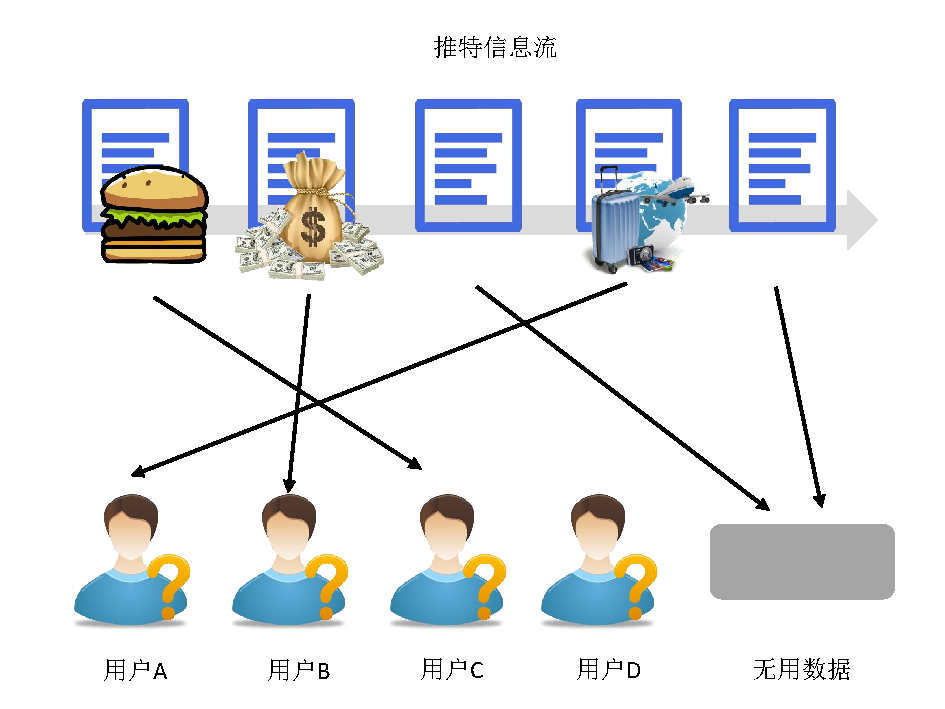
\includegraphics[width=0.8\textwidth]{twitter_search}
  \caption{社交网络平台中信息的实时个性化搜索示意图}
  \label{fig:twitter_search}
\end{figure}

为了解决针对不同用户,为其实时地搜索出相关性强、高质量的信息,许多已有的个性化推荐\upcite{Xie2015Personalized,sontag2012probabilistic,wang2013personalized,tang2015personalized} 以及协同搜索\upcite{liang2014Collaborative,vosecky2014collaborative,xue2009user,yang2014survey} 的工作对这个问题进行了一定的研究。但是很少有面向社交网络个性化搜索的研究,特别是对于实时搜索推荐技术的研究。目前已有的机器学习、自然语言处理、信息检索、人工智能等研究对于社交网络中的实时个性化搜索问题提供了许多帮助。文本分类以及排序的研究\upcite{canuto2015efficient,severyn2015learning,ren2014hierarchical,paik2013novel} 能够为了社交网络中的信息检索提供支持。同时,查询分析以及优化技术\upcite{gao2013query,Letelier2012Static,si2014users} 能够使得信息检索有着显著的提升。

然而,社交网络的环境与传统的新闻、论坛等Web环境有着较大的区别。因此,为了满足社交网络中用户获取信息的需求,这将需要建立新的模型、研究新的方法来解决这一问题。在社交网络中,实现信息的个性化实时推荐面临的主要挑战可以总结如下:
\begin{itemize}
  \item \textbf{信息海量性},在社交网络中,信息产生的速率快,网络中的每一个用户同时扮演着信息生产者、信息传播者和信息接收者的角色。如此高容量的信息流需要一个新的模型来适应持续不断变化的语义特征。
  \item \textbf{主题多样性},社交网络中的信息内容包罗万象,覆盖了许许多多的领域和话题。如果主题模型不能区分众多的话题,这将导致噪声的引入以及不准确的话题模型以及用户模型。
  \item \textbf{数据稀疏性},在社交网络中,信息在不同的主题上的分布是不均匀的,在某些主题上信息量大,而在某些主题上信息是稀疏的。有效的主题模型需要解决数据稀疏性所带来了的影响。
  \item \textbf{社交互动性},社交网络中的用户之间有着丰富的互动信息,与传统的文本信息不同,社交网络中的信息包含了许多有价值的结构化的社交属性。适当地利用这些社交属性能够提高搜索的性能,但是这需要对这些社交属性进行相关性的选择。
\end{itemize}

为了解决上述面临的挑战,本章提出了一种基于语义扩展和文本质量的实时个性化搜索框架,该框架综合考虑了用户的偏好、语义特征和社交属性。首先,本章基于语义扩展提出了一种布尔逻辑关键词过滤(Boolean Logic Keyword Filter)的用户模型。该模型依靠外部搜索引擎提供的知识进行建立,建立的用户模型充分利用了查询扩展以及检索结果的重排序来提高推荐结果的相关性。最终的实验评估证明该模型显著地提高了检索的召回率。此外,本章还基于逻辑回归提出了一种文本质量模型,该模型利用推文的社交属性来评估其文本的质量。该模型能够对推文的文本内容,是否受到大众的认可等进行评估,因此它能帮助系统返回高质量的推文。最终的实验评估证明该模型显著地提高了检索结果的排序性能。

\section{相关定义}
\label{sec2:definition}
本节首先将对社交网络中的实时个性化搜索的任务进行定义,并将其形式化,然后对TREC 2015 Microblog Track的具体任务进行描述。

社交网络中的实时个性化搜索任务可以描述如下。在社交网络中平台中,令信息流表示为$\mathbf{T}$,信息流在社交网络中随着时间不断地产生,信息流$\mathbf{T}$中包含许多种类的话题。令$\mathbf{P}$表示用户集合,每一个用户$p_i \in \mathbf{P}$表示着用户感兴趣的一个话题,用户的兴趣爱好可以通过文本等形式来表示。则社交网络中的实时个性化搜索任务可以定义如下,
\begin{mydef}[实时个性化搜索]\label{def:realPrnzdSearch}
在社交网络中,给定信息流$\mathbf{T}$以及用户集合$\mathbf{P}$,实时个性化搜索的目的是针对不同的用户兴趣爱好$p_i \in \mathbf{P}$,自动地实时地为其推荐高质量的、相关的信息。
\end{mydef}

根据定义\ref{def:realPrnzdSearch}可知,社交网络中的实时个性化搜索需要解决的几个核心关键问题如下。首先是如何表示信息流与用户,其次是如何实现实时推荐,以及如何保证信息的高质量和高相关性。社交网络平台中信息的实时个性化搜索任务可以通过图\ref{fig:real-timeSearch}来表示。
\begin{figure}[!htbp] % use float package if you want it here
  \centering
  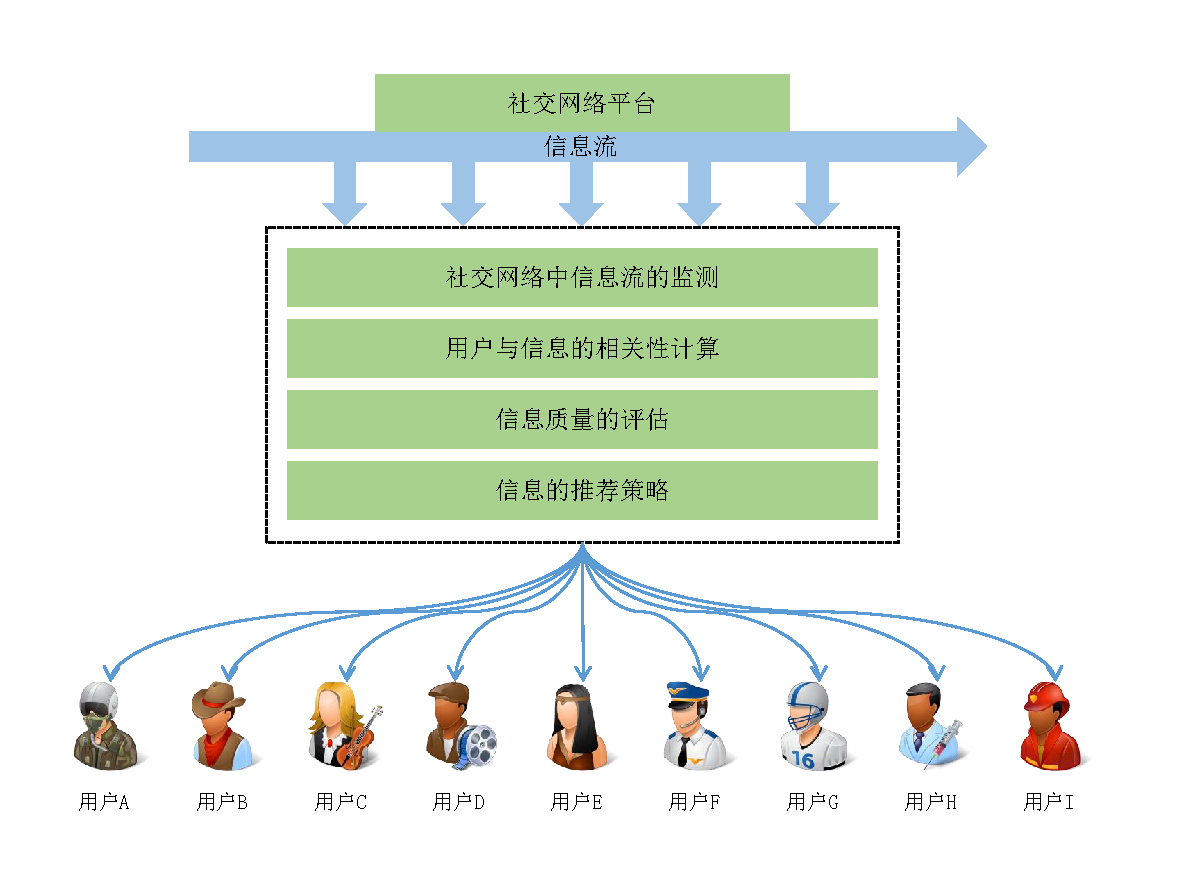
\includegraphics[width=\textwidth]{real-timeSearch}
  \caption{社交网络平台中信息的实时个性化搜索任务图}
  \label{fig:real-timeSearch}
\end{figure}

任务首先要求系统能够实时地监测社交网络中的信息流,然后对不同的用户建立兴趣模型,分析信息与用户之间的相关性。同时任务还要求系统能够对信息的质量做出评估,包括真实性、内容丰富性等。最后,系统需要采取一个良好的推送策略,使得用户不至于淹没在信息中。

TREC 2015 Microblog Track的任务目标是\textbf{实时信息流过滤},实质上也是实时个性化搜索的一种形式。在Microblog Track中,实时信息流过滤的任务目标是根据不同用户的兴趣模型来监测社交媒体中的信息流。值得注意的是,上述的兴趣模型的概念是不同于传统的临时查询。该场景中,交互流程不是用户输入一次查询,然后系统返回结果给用户。该场景不存在实际的查询,取而代之的是系统根据用户的兴趣模型主动地推送\textbf{有趣的}信息给用户。

什么样的信息是有趣的可以考虑如下两个实际的任务模型来帮助更好地理解。
\begin{itemize}
  \item \textbf{场景A:即时性信息推送},在场景A中,用户是定位在使用移动设备的场景,用户可以即时地查看消息。系统基于用户的兴趣模型来判别消息之于用户是否是有趣的,被系统判别为有趣的信息将实时地推送到用户的移动设备(例如手机、平板等)。场景A中的任务目的是上述的推送需要在消息产生的相对较短的时间内完成,该场景中的信息假设是相对较短的。
  \item \textbf{场景B:周期性邮件摘要},在场景B中,用户是定位在使用固定设备的场景,用户周期性的查看消息。与场景A相同,统基于用户的兴趣模型来判别消息之于用户是否是有趣的。但是被系统判别为有趣的信息将被聚集成一个邮件摘要,并且周期性的推送给用户。该场景中的每一个单一信息假设是相对较短的,聚集成的邮件摘要可能很长,我们可以认为这是\textbf{个性化头条新闻}。
\end{itemize}

两个场景都假设推送给用户的消息相对较短,是短消息。因此,推送的消息是否有趣可以根据用户阅读消息的长度或者条数来进行衡量。可以看出,TREC 2015 Microblog Track的任务目标是在两种不同的场景中来考虑社交网络平台中信息的实时个性化搜索问题。

任务中的推文信息(即定义\ref{def:realPrnzdSearch}中的\textbf{T})一条推文以JSON格式保存,字段信息如表\ref{tab:tweetJSON}所示。
\begin{table}[!htbp]
\centering
\caption{推文JSON数据的部分字段信息}
\begin{tabular}{|p{4cm}|p{7cm}|}
\hline
\textbf{字段} & \textbf{描述} \\
\hline
$created\_at$ & 推文发布的时间戳\\
\hline
$id$ & 推文的ID\\
\hline
$text$ & 推文的文本信息\\
\hline
$source$ & 推文的发布终端\\
\hline
$in\_reply\_to\_status\_id$ & 回复的推文的ID\\
\hline
$user$ & 发布推文的用户信息\\
\hline
\end{tabular}
\label{tab:tweetJSON}
\end{table}

表\ref{tab:tweetJSON}中$created\_at$是推文创建的时间,即发布时间。$id$是推文的ID,是唯一的。$text$是推文的文本信息,为短文本,不超过140个字符,可能存在超链接。$source$是推文的发布平台,例如推特Web端,推特手机端,或者通过其他的平台转发至推特等。$in\_reply\_to\_status\_id$是指该推文是否为转发回复其他的推文,如果不是则字段为$null$,如果是则为转发的推文的ID。$user$是指发布推文的用户,也是一个JSON格式的数据,其字段内容在表\ref{tab:userJSON}中给出。
\begin{table}[!htbp]
\centering
\caption{用户JSON数据的部分字段信息}
\begin{tabular}{|p{4cm}|p{7cm}|}
\hline
\textbf{字段} & \textbf{描述} \\
\hline
$created\_at$ & 用户创建的时间戳\\
\hline
$id$ & 用户的ID\\
\hline
$screen\_name$ & 用户的名称\\
\hline
$location$ & 用户的地理信息\\
\hline
$description$ & 用户的自我描述\\
\hline
$followers\_count$ & 用户的粉丝数\\
\hline
$friends\_count$ & 用户的好友数\\
\hline
$favourites\_count$ & 用户收藏推文的数目\\
\hline
$statuses\_count$ & 用户发布推文的数目\\
\hline
$utc\_offset$ & 用户所在时区\\
\hline
$profile\_image\_url$ & 用户的头像\\
\hline
$lang$ & 用户的语种\\
\hline
\end{tabular}
\label{tab:userJSON}
\end{table}

表\ref{tab:userJSON}中$created\_at$为用户账号建立的时间。$id$为用户的ID,是唯一的。$screen\_name$为用户的名字。$location$为用户的地理位置,由用户自己填写。$description$为用户对自己的描述,为一段文本信息。$followers\_count$为用户的粉丝数,即关注该用户的用户数。$friends\_count$为用户的好友数,即用户关注的用户数目。$favourites\_count$为用户收藏的推文的数目。$statuses\_count$为用户历史上发布推文的数目。$utc\_offset$为用户所在的时区的偏差值,单位为秒。$profile\_image\_url$为用户的头像,如果用户没有自定义头像,则为系统默认头像。$lang$为用户的常用语言。

任务中的用户查询(即定义\ref{def:realPrnzdSearch}中的\textbf{P})也是按照JSON格式保存,字段信息如表\ref{tab:queryJSON}所示。
\begin{table}[!htbp]
\centering
\caption{用户查询JSON数据的部分字段信息}
\begin{tabular}{|p{4cm}|p{7cm}|}
\hline
\textbf{字段} & \textbf{描述} \\
\hline
$topic\_id$ & 用户查询的ID\\
\hline
$title$ & 用户查询的标题\\
\hline
$desc$ & 用户查询的描述\\
\hline
$narr$ & 用户查询的详情\\
\hline
\end{tabular}
\label{tab:queryJSON}
\end{table}

其中$topic\_id$为用户查询的ID,即用来标志一个用户感兴趣的话题。$topic\_id$为用户查询的标题,为一个简短的句子。$desc$是用户查询的描述,为文本信息,描述用户所需要的信息。$narr$是用户查询的详情,详细地介绍了用户对于信息需求的细节。

本节介绍了任务的定义以及相关的背景知识,包括推文信息的格式,用户的格式以及用户查询的格式等信息。
%在实时信息流过滤任务中,信息即为推文。在测评阶段,进行测评的系统将监测推特的实时样本信息流并根据用户的兴趣模型(相当于特定的话题)来识别有趣的信息。为了描述的简洁性,我们将上述过程称之为\textbf{兴趣用户的追踪}。

\section{方法描述}
\label{sec2:method}
在本节中,我们设计了一个面向社交网络的实时信息流推荐的系统框架。首先,与传统的信息检索系统相似,推文信息以及用户查询的语义特征被提取出来,数据的预处理用于过滤掉此阶段中无用的信息。其次,为了计算推文信息与用户查询之间的相似度(即相关性),基于外部语料库训练得到的词向量模型来表述提取的特征。除此之外,系统将文本的质量也考虑在内。高质量的文本往往包含高质量的信息,本节提出了一个基于逻辑回归模型的文本质量评估算法来对文本的质量进行衡量。然后,基于得出的相关性与质量,系统针对不同的用户查询对推文信息进行评估。一条相关的、有意思的信息将被归类到最相关的类别中,即归类到最相关的用户查询。最后,为了避免信息洪流、保持消息推送的实时性,本节提出了一个动态的推送策略。因此,用户将实时地收到相关性强、质量高的信息,并且能够避免淹没在信息中。

\subsection{系统框架}
\label{subsec2:systemOverview}
目前在社交网络中,用户只能接收到其关注用户的信息推送,而且这些信息只是简单的按照时间进行排序。理想的搜索系统应当能够分析用户的兴趣爱好,并且自动地推送相关的、高质量的信息给用户。为了满足这一需求,一个面向推特的实时个性化搜索系统的框架设计如图\ref{fig:systemFramework}所示。
\begin{figure}[!htbp] % use float package if you want it here
  \centering
  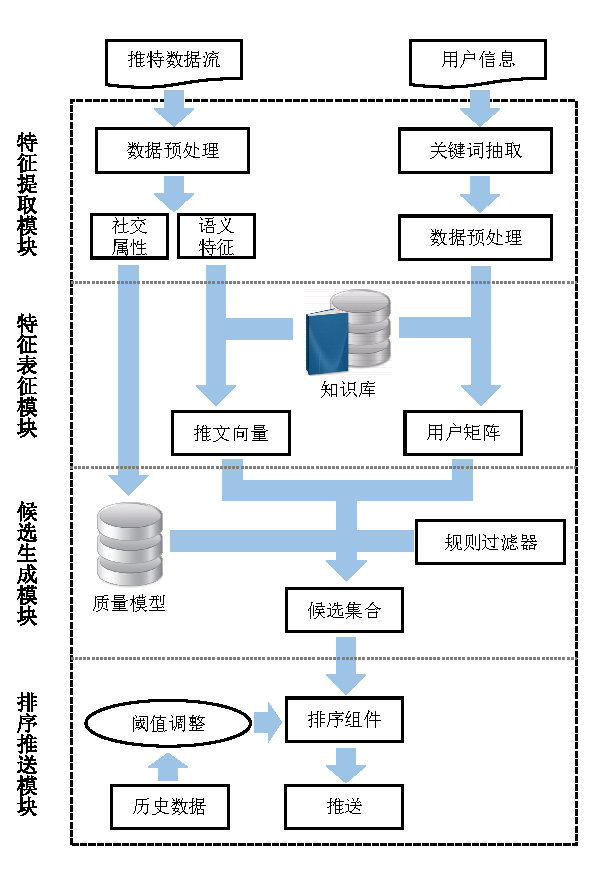
\includegraphics[width=0.7\textwidth]{systemFramework}
  \caption{实时个性化搜索系统框架图}
  \label{fig:systemFramework}
\end{figure}

如图所示,系统主要包括四个主要的模块,分别如下所示。
\begin{itemize}
  \item \textbf{特征提取模块},该模块监测推特信息流,并且接收用户的搜索请求。值得注意的是,在实时个性化搜索任务中,用户的搜索请求相当于某个话题内容的订阅。用户事先输入搜索后,在相关的信息发布时实时推送给用户。推特信息流通过TREC-API\footnote{\url{https://github.com/lintool/twitter-tools}}工具监测。用户的搜索由官方提供,以$p_i \in \textbf{P}$表示。在特征提取之前,数据的预处理将用来过滤掉无用的信息。对于推特信息流,系统提取其语义特征以及社交属性;对于用户查询,系统提取搜索中的关键词作为基础特征。
  \item \textbf{特征表征模块},该模块通过几种技术来扩展及表征所提取的语义特征。推文信息以及用户查询通过该模块进行了语义增强,该模块使得推文以及用户之间的相关度计算更加的方便。
  \item \textbf{候选生成模块},该模块通过语义特征以及社交属性将推文分类到与之最相关的用户。这一过程同时考虑了相关性以及推文的质量,因此用户收到的信息不仅是有趣的而且是高质量的。
  \item \textbf{排序推送模块},该模块通过最终的得分来对每个用户的推文候选队列进行排序,并且利用历史数据进行阈值的动态调整。该模块能够保证用户不错过重要的高质量的信息,又不至于淹没在过多的信息中。
\end{itemize}

在之后的小节中,我们将详细地介绍每一个模块应用的算法以及实现。

\subsection{特征提取模块}
\label{subsec2:feaureExtraction}
推文信息依靠监测推特的抽样信息流来获取\upcite{wang2015assessor}。在获取到推文后,数据的实时预处理用来过滤掉此阶段内无效的信息,减少无意义的以及冗余的信息。推特数据流上的相关数据预处理方法包含如下一些技术,
\begin{itemize}
  \item \textbf{语言识别},根据任务要求,非英文的推文将被直接过滤掉来简化问题的复杂度。本系统中使用的工具为\textbf{无限元模型语言识别}(\textit{Language Detection with Infinity Gram}),简称为ldig\footnote{\url{https://github.com/shuyo/ldig}}。ldig工具是一个针对短文本消息(例如推特)的语言识别器,能够支持对于17种语言的识别,准确率达到了99.1\%。除此之外,系统还使用了基于字符编码集的语言识别方法来区分英文句子和非英文句子。通过训练得出一个阈值,包含英文字符多的推文将被保留,其余的将被过滤掉。
  \item \textbf{冗余过滤},社交网络中由于复制,转发等行为使得相同信息的推文存在着很多的冗余,如果不进行冗余过滤,那么将会有很多相同的内容推送给用户,使得用户淹没在重复的信息中。因此,对于内容相同或者相似的推文,系统只保存一个副本。为了实现该目标,一种方法是利用表\ref{tab:tweetJSON}中提到的推文$id$字段和$in\_reply\_to\_status\_id$字段来识别冗余信息。如果推文是原创信息,则我们记录其$id$值;如果推文是转发信息,则可以检查该推文转发推文的$id$是否已经存在来判别是否是冗余信息。每当一条新的推文被爬取时,首先来检查推文的$id$来做冗余消除。该方法简单有效,能够迅速滤除掉大部分的冗余信息。但是当推文是复制其他推文的信息或者做出微小的改动,则该方法无法识别。因此,另外一种冗余消除技术,$simhash$技术被应用。$simhash$技术是用于处理网页冗余的技术,该方法将一个文档转换成一个数字指纹(即一串定长的0-1编码),被称为\textbf{哈希相似码}。两个文档的哈希相似码之间的汉明距离(\textit{hamming distance})越短,则说明两个文档之间的相似度越大。哈希相似码的计算公式如下所示,
  \begin{equation}
  \label{simhash}
    {\mathbf{s}_{hash}} = sign(\sum\nolimits_{i = 1}^n {{w_i} \cdot {\mathbf{c}_i}} )
  \end{equation}
其中$\mathbf{c}_i$是第$i$个词的哈希码,为一个定长的向量,$w_i$是该词的权重,为标量,$sign$是是一个符号函数,让结果向量中的每一个比特的正数位变成1,负数位变成0。simhash算法的过程大概如下。首先,对文档进行关键词抽取,得到特征$\mathbf{c}_i$和权重$w_i$。然后,对所有特征进行加权的位计算。最后,对得到的结果进行哈希码的生成,这个产生值和具体采用的算法有关,这里采用的一个简单的符号函数。将推文转换成哈希相似码后,我们就可以利用推文之间的汉明距离来判别推文间的相似性,来进行冗余消除。基于推文的$id$进行冗余消除是一种高效的方法,能够解决大多数情况下的问题,但是对于复制或者修改的内容无法识别。simhash算法是基于推文的内容进行冗余消除,能够有效地解决内容相似的推文冗余,但是相比于基于推文$id$的方法耗时会长一些,因为计算哈希相似码的过程将会有额外的计算量。在本章提出的系统中,两种算法被结合起来完成冗余消除。首先利用基于推文$id$的方法进行粗的冗余消除,如果无法判别则计算推文的哈希相似码后,根据汉明距离进行判别。
\end{itemize}

在数据的预处理后,我们将推文信息和用户查询的语义特征和社交属性抽取出来。对于推文,名词以及动词是句子中最重要的部分。因此,退文中的名词以及动词(除去停用词)被抽取出来作为语义特征,并且每一个词都根据其在句子中的重要性得到一个不同的权重。一条推文的语义特征可以表示成$\mathbf{ts} = \{ {w_1}{\mathbf{t}_1},{w_2}{\mathbf{t}_2},\cdots,{w_n}{\mathbf{t}_n}\}$,其中$\mathbf{ts}$表示一条推文,$\mathbf{t}_i$表示一个词语,$w_i$为该词语的权重。词语的权重与该词语在句子中的位置、出现的频率等有关。

由于社交网络信息提供了丰富的社交行为属性,社交属性可以被用于评估推文的真实性和质量。推文是按照JSON格式存储的,因此获取系统所需的社交属性是非常便捷的,例如发布推文的用户、推文的转发量、推文的评论数、推文的URL数、推文的标签、推文中有意义的词数、推文的长度等等。这些信息都可用于进行训练,来评估推文的质量。

\begin{figure}[!htbp] % use float package if you want it here
  \centering
  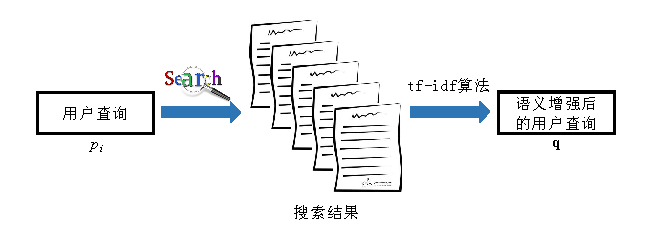
\includegraphics[width=0.9\textwidth]{semanticExp}
  \caption{用户查询的语义扩展示意图}
  \label{fig:semanticExp}
\end{figure}

对于用户查询,对用户的兴趣爱好描述被当成一个查询,如表\ref{tab:queryJSON}所示。系统对查询进行分析,计算用户所感兴趣的推文。首先,用户查询中的关键词如同推文一样的被提取出来。但是,用户查询往往比较简短,表述能力是有限的。短文本的检索面临着词语失配的问题,即用户查询与推文信息的词语重叠相对较少,这将导致很多描述着同一事件的文本因为使用了不同的词汇而检索失败。为了解决该问题,语义扩展方法往往被用于增强检索的性能。语义扩展方法主要分成两大类,基于搜索引擎的语义扩展和基于知识库的语义扩展。本节中系统使用的是基于搜索引擎的语义扩展技术来丰富查询的信息,大致流程如图\ref{fig:semanticExp}所示。在第一步中提取出来的关键词被当做搜索引擎的输入。返回的top-k个结果的摘要文本部分被收集用来做下一步的计算,每一个返回的结果都包含若干个词语。在整个结果集中可以使用tf-idf算法可以被用来计算每一个词语的权重。针对每一个用户查询,一个带有tf-idf值的词语列表被计算返回。语义增强后的用户查询可被写作$\mathbf{q} = \{ {\mathbf{k}_1}:{v_1},{\mathbf{k}_2}:{v_2},...,{\mathbf{k}_n}:{v_n}\}$,其中$\mathbf{k}_i$表示关键词,$v_i$表示词语$\mathbf{k}_i$的tf-idf值。

\subsection{特征提取模块}
\label{subsec2:featureRep}
已有的工作对语义特征的表示模型有着很多的研究,例如\textbf{词袋模型}(\textit{Bag of Words Model})等。词袋模型忽略了文本的语法和词序,仅仅将文本当作词语的聚集。该模型假设每一个词是独立的,即文本中词的概率与上下文是无关的,它简化了表示方法,但是忽略了语法和词序,在某些情况下带来了一些缺陷。基于此的一些改进算法,例如二元词袋模型、三元词袋模型等在一定程度上解决了这些缺陷。然而,词语失配问题仍然是词袋模型无法解决的问题。

为了解决词语失配问题,\textbf{词向量模型}(Word Vector Model)被提出来表示语义特征。使用\textit{word2vec}技术来对词语进行向量化,\textit{gensim}\footnote{\url{http://radimrehurek.com/gensim/index.html}}是一个比较方便的工具来处理该问题。为了训练词向量模型,维基百科的英文预料库被用于训练\footnote{\url{https://dumps.wikimedia.org/enwiki/20160113/}}。图\ref{fig:real-timeSearch}中的知识库基于维基百科英文语料库使用\textit{gensim}工具训练得到。推文$\mathbf{ts}$中的每一个词语$\mathbf{t}_i$,可被表示成一个向量$\mathbf{t}_i=\left(\alpha_1,\alpha_2,\cdots,\alpha_m\right)^T$,其中$m$为词向量模型设置的维度(例如200、400等),参数$\alpha_j$表示词向量第$j$维的值。因此,一条推文$\mathbf{ts}$可向量化为$\mathbf{ts}= \sum w_i \mathbf{t}_i$,其中$w_i$为词语$\mathbf{t}_i$的权重。与处理推文的方式相似,语义增强后的用户查询$q$中的每一个关键词$\mathbf{k}_i$可以表示成$\mathbf{k}_i = \left(\beta_1,\beta_2,\cdots,\beta_m\right)^T$,其中参数$\beta_j$为关键词$\mathbf{k}_i$第$j$维的值。而且语义增强后的用户查询$\mathbf{q} = \sum v_i \mathbf{k}_i$,$v_i$为词语$\mathbf{k}_i$的权重。按照上述流程,推文信息以及用户查询通过词向量模型转化成了向量形式。

\subsection{候选生成模块}
\label{subsec2:candidate}
依靠词向量模型,词语的失配问题得到了比较好的解决。但是该方法也是一把双刃剑,词向量模型在获取更多相关的信息的时候也会带来许多低相关的信息给用户,即词向量模型在提高召回率的时候降低了准确率。为了解决该问题,系统使用了一个规则过滤器\textbf{布尔逻辑关键词模型}(\textit{Boolean Logic Keyword Model})来提高准确率。布尔逻辑关键词模型将用户查询表示成如下形式,
\begin{equation}
\label{eq:blkm}
  p = \{1:\left(\mathbf{t}_1 || \mathbf{t}_2\right) \& \& \left(\mathbf{t}_3 || \mathbf{t}_4\right),~~0:\mathbf{t}_5 || \mathbf{t}_6\}
\end{equation}
其中$p$代表一个用户查询,其中包含两个域1和0。值为1的域代表着该用户查询检索到的结果中必须出现的词,值为0的域代表着该用户查询检索到的结果中不一定须要出现的词,但是命中会增加推文信息和用户查询之间的相关性。符号$||$表示逻辑上的“或”关系,代表多个词出现某一个即可;符号$\&\&$表示逻辑上的“与”关系,代表多个词须要同时出现才满足。例如公式(\ref{eq:blkm})表示能够通过过滤器的推文中必须包含词语$t_1$或者$t_2$,并且包含$t_3$或者$t_4$。如果推文中包含$t_5$或者$t_6$,则会增加推文信息与用户查询之间的相关性。系统根据语义扩展后的用户查询中的词语的tf-idf值来生成规则过滤器。我们为规则过滤器设置两个参数阈值$\eta$和$\gamma$($\eta < \gamma$)。假设tf-idf$_{max}$表示一个用户查询$p$中的最大tf-idf值。则阈值$\gamma$设置为0.7$\cdot$tf-idf$_{max}$,阈值$\eta$设置为0.9$\cdot$tf-idf$_{max}$,这是一个经验性的参数设置。对于tf-idf值大于$\eta$的词语将被加入到$p$中域为1的列表中,对于tf-idf值大于$\gamma$又小于$\eta$的词语将被加入到$p$中域为0的列表中,对于tf-idf值小于$\gamma$的词语将不作处理。

所有从推特信息流中监测到的推文首先都会经过根据布尔逻辑关键词模型生成的规则过滤器。如果推文不与任何规则过滤器匹配,则该条推文将被直接丢弃。如果推文通过了某个规则过滤器,则推文信息与该用户查询之间的语义得分讲根据它们之间的相似度计算得出。然后推文将根据公式(\ref{eq:blkm})以及语义得分分类到某一个用户查询中。已有的研究主要有两类计算语义得分的方法来评估推文信息与用户查询之间的相关性。
\begin{itemize}
  \item \textbf{基于tf-idf的相似度},根据推文信息和用户查询生成的向量以及tf-idf权重进行相似度计算,计算公式如下所示,
  \begin{equation}
  \label{eq:tf-idf}
  sim = \frac{\mathbf{ts}^T \cdot \mathbf{q}}{\|\mathbf{ts}\| \cdot \|\mathbf{q}\|} = \frac{\left(\sum \limits_{i=1}^m {w_i \mathbf{t}_i}\right)^T \cdot \sum \limits_{j=1}^m {v_j \mathbf{k}_j}}{\sqrt{\left(\sum \limits_{i=1}^m {w_i \mathbf{t}_i}\right)^T \left(\sum \limits_{i=1}^m {w_i \mathbf{t}_i}\right)}\sqrt{\left(\sum \limits_{j=1}^m {v_j \mathbf{k}_j}\right)^T \left(\sum \limits_{j=1}^m {v_j \mathbf{k}_j}\right)}}
  \end{equation}
  其中$\mathbf{ts}$表示推文信息的向量,$\mathbf{q}$表示用户查询的向量。$w_i$为词向量$\mathbf{t}_i$的权重,$v_j$为词向量$\mathbf{k}_j$的权重。
  \item \textbf{基于BM25的相似度},利用算法Okapi BM25的权重函数来评估推文信息和用户查询之间的相似度。算法Okapi BM25是一个基于词袋模型的算法,根据文档中出现的查询词的频率进行权重计算。推文信息与用户查询之间的相似度计算如下,
  \begin{equation}
  \label{eq:bm25}
  sim = \sum \limits_{q_i \in Q} {idf\left(q_i\right) \cdot \frac{ f\left(q_i,D\right) \cdot \left(k_1 + 1\right)}{f\left(q_i,D\right) + k_1 \cdot \left(1-b+b\cdot\frac{|D|}{avgdl}\right)}}
  \end{equation}
  其中$D$表示一个文档,即一条推文信息,$Q$表示用户查询。函数$f\left(q_i,D\right)$表示查询词$q_i$在文档$D$中的词频,$|D|$表示文档$D$的长度,$avgdl$表示文档集中文档的平均长度,$k_1$以及$b$为调整参数。系统一般经验性的设置$k_1=2$,$b=0.75$。
\end{itemize}

以上是系统对推文信息和用户查询之间相关性的处理,下面介绍系统对于推文的质量的评估。在特征提取模块中抽取的社交属性可被用来训练推文的\textbf{质量模型}(\textit{Quality Model})。我们首先人工地标注推文的质量得分,标注不依据推文的类别,单纯考虑推文是否能够带来信息量。质量高的推文标注1,质量低的推文标注0。如果推文能提供更多的信息,并且撰写得更完整,则推文会获得高的得分。我们使用\textbf{逻辑回归模型}(\textit{Logistic Regression Model})来对文本的质量模型进行建模,模型如下所示,
\begin{equation}
\label{eq:lr}
  h_ {\bm{\theta}} \left(\mathbf{x}\right) = \frac{1}{1 + e^{-{{\bm{\theta}}^T}\mathbf{x}}}
\end{equation}
其中$\mathbf{x}=\left({x_1},{x_2},\cdot,{x_n}\right)$是抽取的社交属性,$\bm{\theta}=\left({\theta _1},{\theta _2},\cdot,{\theta _n}\right)$为待训练的参数。实现一般来说,用户更倾向于接受文本质量高的、由权威发布的信息,基于以上假设,我们选取如下的社交属性作为特征。
\begin{itemize}
  \item \textbf{用户粉丝数}(\textit{FollowerCnt}),表示发布推文信息的用户的粉丝数。粉丝数高的用户表示该用户在社交网络中是受欢迎的,因此该用户发布的推文信息很大概率上是高质量的信息。
  \item \textbf{用户推文数}(\textit{StatusCnt}),表示发布推文信息的用户历史上发布的推文数。用户发布推文的数目预示着用户的活跃度,而一个活跃的用户更可能发布高质量的信息。
  \item \textbf{推文转发数}(\textit{RetweetCnt}),表示推文的转发数。一条推文的转发数越大说明这一条推文越受人欢迎,质量越高。
  \item \textbf{推文转发等级}(\textit{RetweetLvl}),表示对转发数使用对数函数后的转发等级。
  \item \textbf{推文点赞数}(\textit{CollectCnt}),表示推文的点赞数。用户如果认为一条推文是吸引人的,信息丰富的,则可以点赞或者收藏。
  \item \textbf{推文词语数}(\textit{WordCnt}),表示推文中除去停用词的文本长度,即词语数。一般来说,长的文本相对于短的文本的信息量会大一些。
  \item \textbf{推文字符数}(\textit{CharCnt}),表示推文中除去停用词的文本的字符数。
  \item \textbf{短链接数}(\textit{UrlCnt}),表示推文中短链接的数目。信息量丰富的文本往往会在推文末尾给出一个短链接。
\end{itemize}

\begin{figure}[!htbp]
   \begin{minipage}{0.48\textwidth}
     \centering
     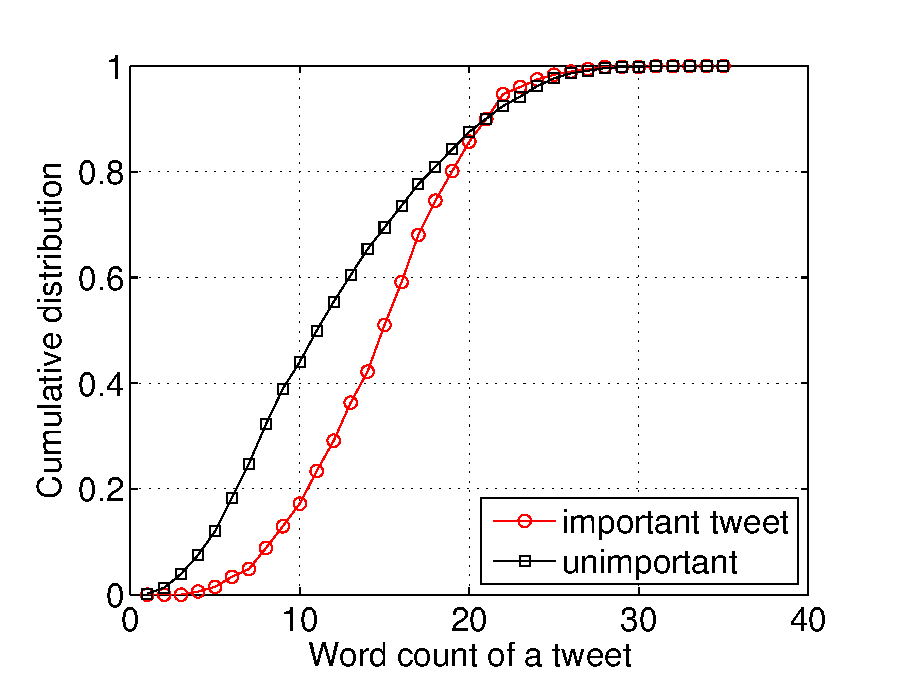
\includegraphics[width=\linewidth]{wordCntCDF}
     \caption{\textit{WordCnt}的累积分布函数}
     \label{fig:wordCntCDF}
   \end{minipage}
   \hfill
   \begin {minipage}{0.48\textwidth}
     \centering
     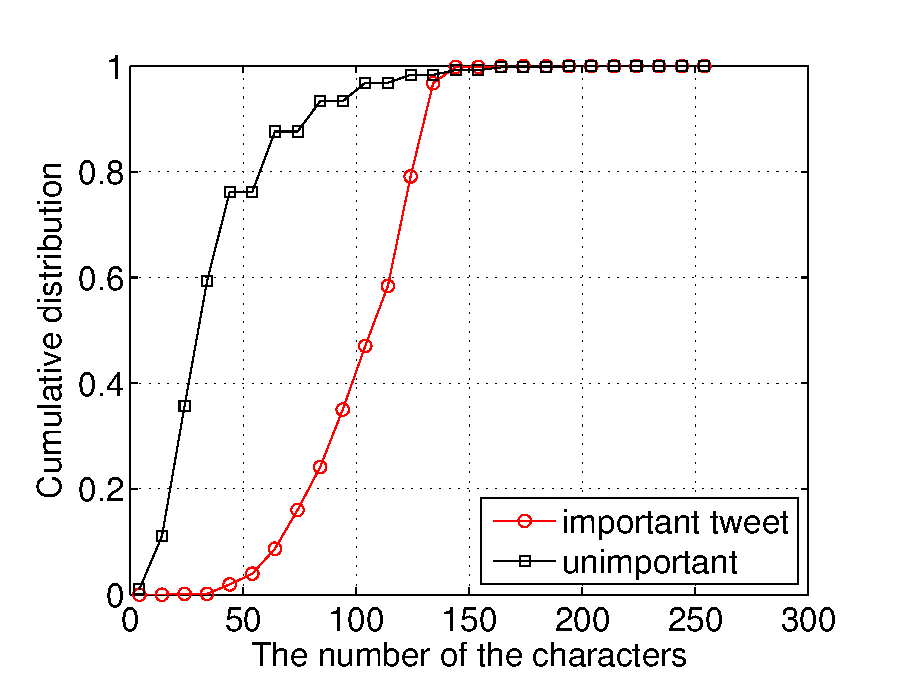
\includegraphics[width=\linewidth]{charCntCDF}
     \caption{\textit{CharCnt}的累积分布函数}
     \label{fig:charCntCDF}
   \end{minipage}
   \\
   \begin{minipage}{0.48\textwidth}
     \centering
     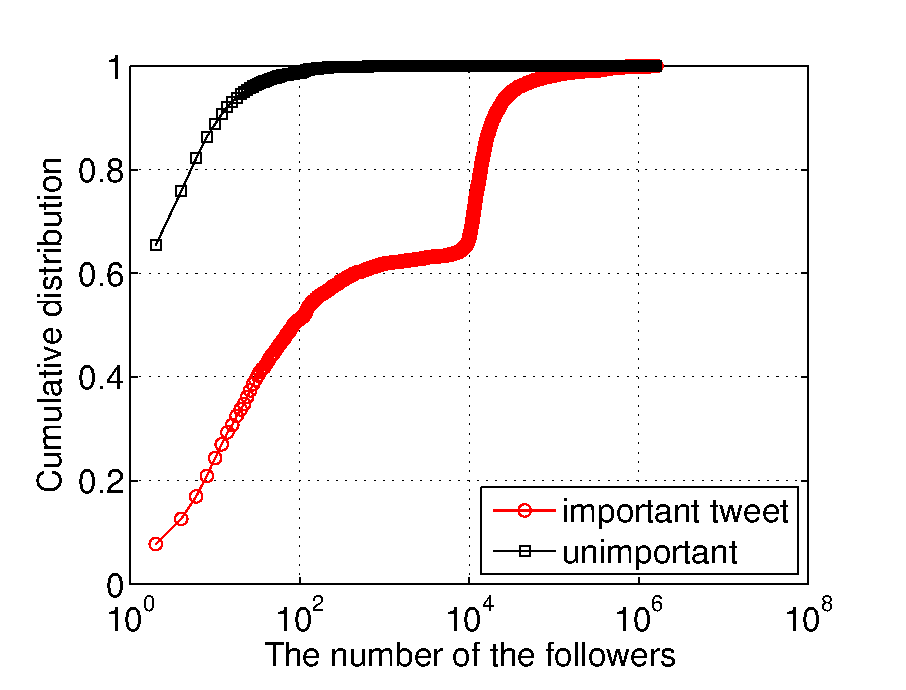
\includegraphics[width=\linewidth]{followerCntCDF}
     \caption{\textit{FollowerCnt}的累积分布函数}
     \label{fig:followerCntCDF}
   \end{minipage}
   \hfill
   \begin {minipage}{0.48\textwidth}
     \centering
     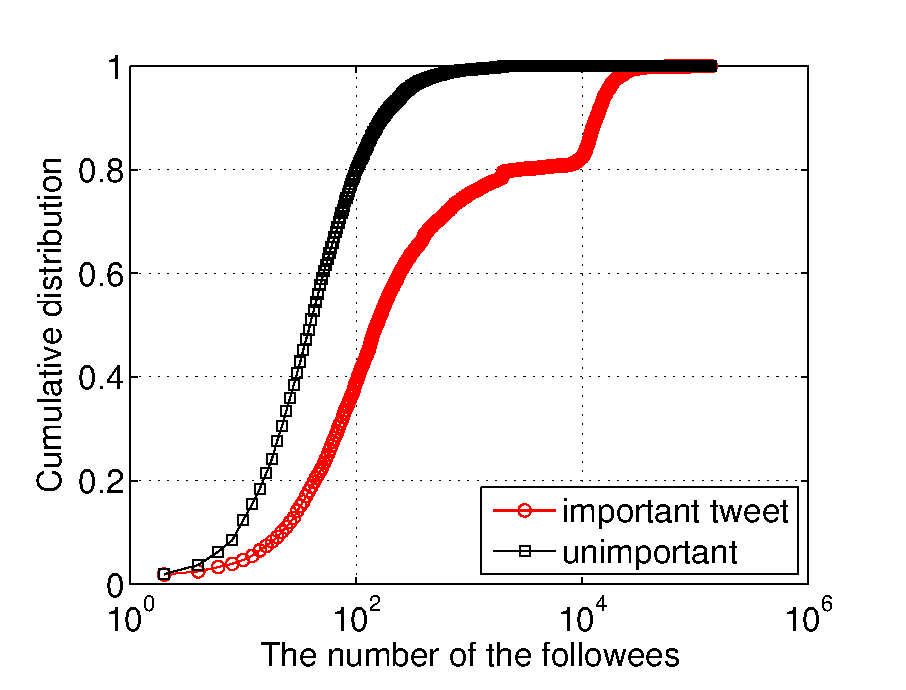
\includegraphics[width=\linewidth]{followeeCntCDF}
     \caption{\textit{FolloweeCnt}的累积分布函数}
     \label{fig:followeeCntCDF}
   \end{minipage}
   \\
   \begin{minipage}{0.48\textwidth}
     \centering
     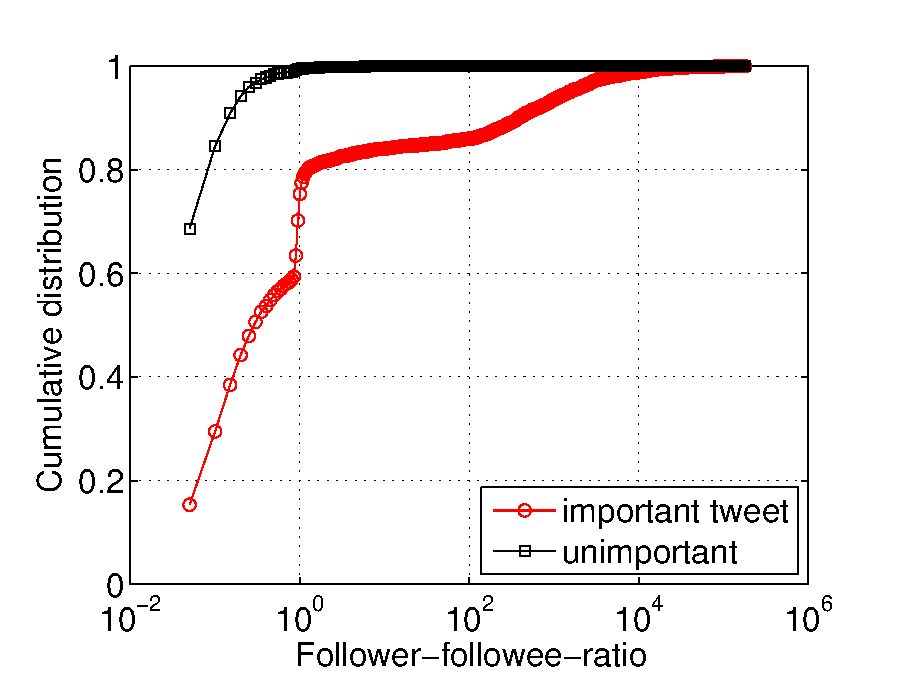
\includegraphics[width=\linewidth]{FFRCDF}
     \caption{\textit{FFR}的累积分布函数}
     \label{fig:FFRCDF}
   \end{minipage}
   \hfill
   \begin {minipage}{0.48\textwidth}
     \centering
     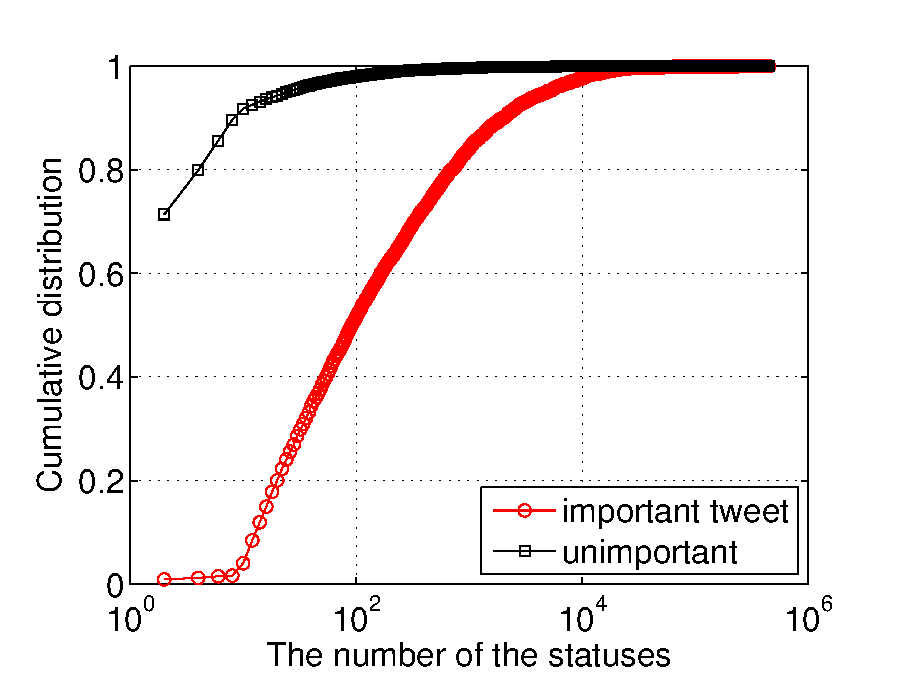
\includegraphics[width=\linewidth]{statusCntCDF}
     \caption{\textit{StatusCnt}的累积分布函数}
     \label{fig:StatusCnt}
   \end{minipage}
\end{figure}

为了检验抽取出来的社交属性的有效性,我们计算了人工标注数据集中的各个社交属性中的\textbf{累计分布函数}(\textit{cumulative distribution function})来进行观察。推文根据其文本质量被标记成1或者0,其中1表示这是一条质量高的推文,反之则表示这是一条质量不高的推文。社交属性的累计分布函数结果如图\ref{fig:wordCntCDF}至图\ref{fig:StatusCnt}所示,两个分类的累计分布函数曲线显示了特征的区分能力。从结果图可知,\textit{CharCnt}、textit{FolloweeCnt}、\textit{FFR}以及\textit{StatusCnt}是区分推文是否高质量的有效的特征。由图\ref{fig:charCntCDF}可知,超过95\%的低质量的推文的字符数都小于100,而超过50\%的高质量的推文的字符数都大于100。由图\ref{fig:followerCntCDF}和图\ref{fig:FFRCDF}可知,拥有高粉丝数和高粉丝-好友比的用户更可能发布高质量的推文。由图\ref{fig:StatusCnt}可知,活跃用户更有可能发布高质量的推文。因此,抽取的社交属性能够被用于训练评估推文质量的分类器。

在计算得到推文信息和用户查询之间的语义相似度和推文的质量得分后,二者被综合起来用来评估推文的最终得分,详细流程在下一个小节中介绍。

\subsection{排序推送模块}
\label{subsec2:scorePush}
基于语义特征和社交属性,我们得到了推文信息和用户查询的语义相似度以及推文的质量得分。以上两种得分的值域为[0,1]。对于一个用户查询,一条推文的最终得分考虑了以上的两个方面,形式化为如下所示,
\begin{equation}\label{fs}
  f\left( \mathbf{ts}, \mathbf{q} \right) = sim \cdot {h_ {\bm{\theta}}} \left(x\right)
\end{equation}
其中$sim$为语义相似度得分,参见公式(\ref{eq:tf-idf})和公式(\ref{eq:bm25})。基于tf-idf和基于BM25算法的语义相似度得分在系统中是可选的。$h_ {\bm{\theta}}$为推文的质量得分,参见公式(\ref{eq:lr})。

当计算完一条推文和各个用户查询之间的分数后,推文将分类到得分最高的用户查询作为候选。候选队列中的推文按照得分$f\left( \mathbf{ts}, \mathbf{q} \right)$进行排序。按照任务需求,如果推文对于一个用户查询是相关的且高质量的,那么系统将把该推文推送给感兴趣的用户。但是如果一直推送给用户信息,那么将导致信息淹没。任务要求系统在保证用户不被信息淹没的情况下,同时实时地推送给用户消息,这是一个约束满足问题。问题可形式化为,用户每天接受信息的数量是一定的,系统需要根据当前队列中的信息来决策何时推送给用户。系统提出了一种\textbf{动态阈值调整算法}来保证相关的高质量的推文及时的推送,且在时间上是均匀分布的。算法根据候一个用户查询的选集队列的历史数据,可以得到一个最高得分$f_{max}$,设计一个梯度阈值函数$\zeta\left(f_{max},t\right)$如下所示,
\begin{equation}
\label{eq:thresholdDynamic}
  \zeta\left(f_{max},t\right) = \left\{ {\begin{array}{*{20}{c}}
{(0.9 - d) \cdot {f_{\max }}}&{d < 0.4}\\
{0.5 \cdot {f_{\max }}}&{d \ge 0.4}
\end{array}} \right.
\end{equation}
其中$d$表示衰减值,且$d = c \cdot floor(t/2)$。式中的$c$表示衰减系数,$floor$为向下取整函数,$t$为一天中的时间,$t \in [0,24]$。观察公式(\ref{eq:thresholdDynamic})可知,阈值的变化与队列中的最高得分$f_{max}$和时间$t$相关。为了得到相关性强、质量高的推文,阈值在一开始时相对较高。在$t=0$时刻,阈值为$0.9 \cdot f_{max}$。为了给用户带来更多更全面的信息,阈值随着时间的变化不断减小。为了避免推送不相关或者低质量的信息,阈值在降低一定程度后不再变化,最终保持在$0.5 \cdot f_{max}$。例如,经验性地设置衰减系数$c=0.05$,当$t=16$时,阈值衰减为$0.5 \cdot f_{max}$后不再变化。动态阈值调整算法的思想是在一开始设置一个相对较高的阈值来获取高质量的推文,然后降低阈值来保证信息的数量。当推文的最终得分超过当时的阈值,则系统将立即推送该信息给相应的用户。由上述的各个模块描述可知,实时个性化搜索算法如算法所示,且阈值将随时间动态变化。
\begin{algorithm}[!ht]
\caption{实时个性化搜索算法}
\label{alg:livePush}
\begin{algorithmic}[1]
  \REQUIRE $\mathbf{T} = \{ \mathbf{ts}_1, \mathbf{ts}_2, \cdots, \mathbf{ts}_N \}$, $\mathbf{P} = \{ p_1, p_2, \cdots, p_M \}$, $Z$
  \ENSURE $\mathbf{R} = \{ \mathbf{R}_1, \mathbf{R}_2, \cdots, \mathbf{R}_M \}$
  \FORALL {$p_i \in \mathbf{P}$}
    \STATE $\mathbf{q}_i = \{ {\mathbf{k}_1}:{v_1},{\mathbf{k}_2}:{v_2},...,{\mathbf{k}_n}:{v_n}\}$
    \STATE $p_i = \{1:\left(\mathbf{t}_1 || \mathbf{t}_2\right) \& \& \left(\mathbf{t}_3 || \mathbf{t}_4\right),~~0:\mathbf{t}_5 || \mathbf{t}_6\}$
  \ENDFOR
  \FORALL {$\mathbf{k}_j$}
    \STATE $\mathbf{k}_j = \left(\beta_1,\beta_2,\cdots,\beta_m\right)^T$
    \STATE $\mathbf{q}_i = \sum v_i \mathbf{k}_i$
  \ENDFOR
  \WHILE {$\left| \mathbf{R}_i \right| < Z$ $\& \& \mathbf{T} = \emptyset$}
    \STATE $\mathbf{ts}_i = pop\left(\mathbf{T}\right)$
    \STATE $\mathbf{ts}_i = \{ {w_1}{\mathbf{t}_1},{w_2}{\mathbf{t}_2},\cdots,{w_n}{\mathbf{t}_n}\}$
    \IF {$\mathbf{ts}_i$ matches $p_j$}
     \FORALL {$\mathbf{t}_k \in \mathbf{ts}_i$}
       \STATE $\mathbf{t}_k=\left(\alpha_1,\alpha_2,\cdots,\alpha_m\right)^T$
     \ENDFOR
     \STATE $\mathbf{ts}_k = \sum w_i \mathbf{t}_i$
     \STATE $f\left( \mathbf{ts}_i, \mathbf{q}_j \right) = sim \cdot {h_ {\bm{\theta}}}\left(x\right)$
    \ENDIF
    \IF {$f\left( \mathbf{ts}_i, \mathbf{q}_j \right) \geq \zeta$}
      \STATE $\mathbf{R}_j = \mathbf{R}_j \cup \mathbf{ts}_i$
    \ENDIF
  \ENDWHILE
\end{algorithmic}
\end{algorithm}

\section{实验分析}
\label{sec2:experiment}
本节中,我们通过TREC 2015 Microblog Track的实时测评对系统进行了多方面的验证。并对实验结果进行了分析。首先,本节介绍了实验的设置,其次介绍了评测标准,最后对实验结果进行了分析。本节中的实验基于八核、16GB内存、SSD硬盘的机器上运行,操作系统为Ubuntu 14.04 64位系统。系统主要基于Python和Java语言实现,Python版本为2.7,JDK版本为1.8版本。

\subsection{数据集及实验环境}
\label{subsec2:dataset}
\begin{figure}[!htbp]
  \centering
  % Requires \usepackage{graphicx}
  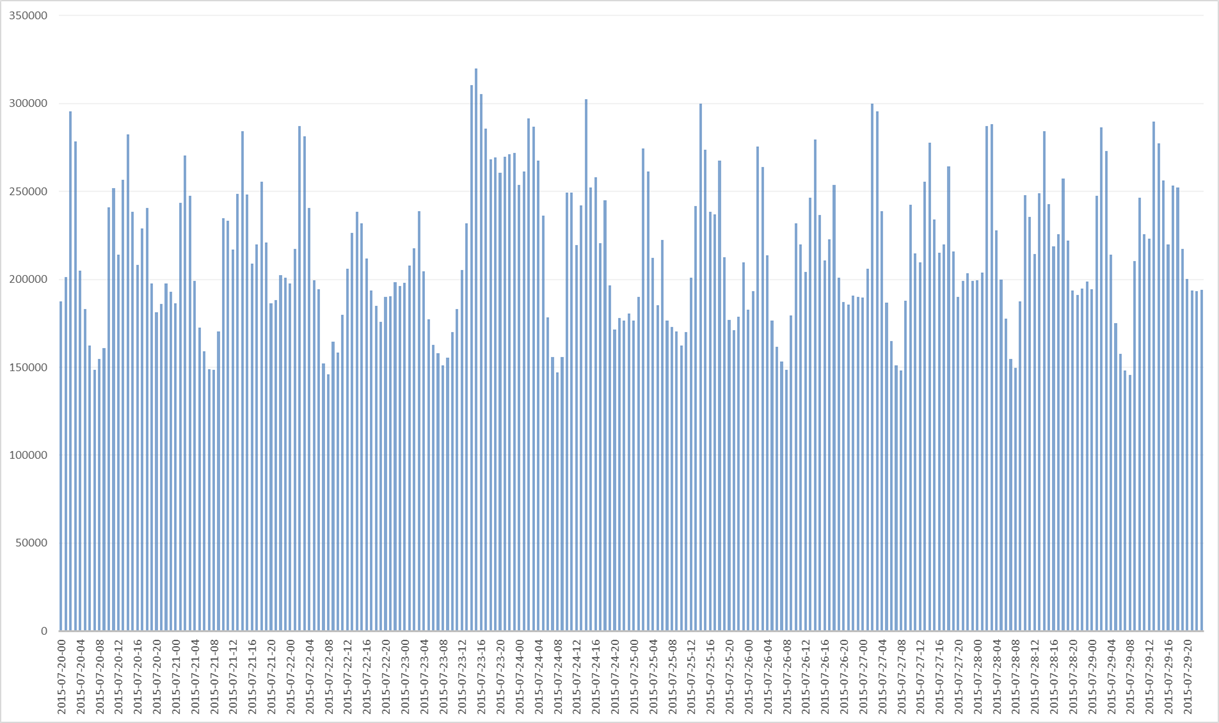
\includegraphics[width=\textwidth]{stream}
  \caption{推特数据流的分布}
  \label{fig:twitterDis}
\end{figure}

为了评估系统的稳定性和算法的有效性,TREC 2015 Microblog Track的实时测评采用了10天的推特信息流数据,时间从2015年07月20日00:00:00 UTC至2015年07月29日23:59:59 UTC,时区为世界标准时间。数据集总共包含51,770,318条真实推文,共有225个用户查询由官方提供。推文的时间分布如图\ref{fig:twitterDis}所示,横轴代表时间,纵轴代表推文的数量。从图中可知,推文的分布具有一定的周期性,周期大约为12个小时。

在评测的时间段内,系统需要保持持续运行来接收推特信息流。系统通过设计的算法,将有趣的、高质量的推文实时地推送给官方设计的用户。在评测结束后,将最终的结果上传至NIST的服务器。为了简化任务,对于两个场景,系统只要求处理英文的推文。在场景A和场景B中的具体的要求如下所示。
\begin{itemize}
  \item \textbf{场景A:即时性信息推送}。在场景A中,系统允许每天推送给一个用户查询至多10条推文。如果对于某个用户查询,系统推送超过10条推文,则NIST只会保存前10条推文。对于每条推文,系统需要记录推文的ID以及系统的推送时间戳。评测标准基于系统的推送时间戳和推文的创建时间戳之间的时间间隔会有惩罚机制。每一个用户查询至多10条的推送是为了适应在移动场景下用户的真实需求,用户每天接收即时信息的推送过于频繁会使得用户淹没在信息中。但是场景A不要求完全按照现实生活中来模拟用户需求,例如用户不希望在半夜接收到推送等等。
  \item \textbf{场景B:周期性邮件摘要}。在场景B中,系统需要针对一个用户查询聚合前100的相关的、高质量的信息。场景B要求系统在一天结束后的相对较短的一段时间内将结果返回给用户,保证用户能够很快地收到结果。
\end{itemize}

场景A中返回结果形式为$(topic\_id,tweet\_id,delivery\_time,runtag)$的四元组,其中$topic\_id$为官方给出的用户查询ID(即话题),$tweet\_id$是推送的推文的ID,$delivery\_time$为系统的推送时间戳,$runtag$为系统的运行标志。场景B中返回结果形式为$(YYYYMMDD, topic\_id, Q0, tweet\_id, rank, score, runtag)$的七元组,其中$YYYYMMDD$为日期,$topic\_id$为官方给出的用户查询ID,$Q0$为TREC默认的一个字符(对系统无影响),$tweet\_id$为推文的ID,$rank$为改推文的排序,$score$为推文的得分,$runtag$为系统的运行标志。
\subsection{评测标准}
\label{subsec2:evalMetrics}
在两个场景中,系统提交的所有结果都会由NIST的评测员独立的进行结果评估。每一条推文都会被评论员按照四挡进行打分,分别为\textbf{垃圾信息},\textbf{不相关},\textbf{相关},\textbf{高相关}。为了简化任务,非英文的推文将直接标记为垃圾信息。如果一条推文中既包含英文信息又包含非英文信息,则由评测员来决定。值得注意的是,评测员会检查推文中的短链接里的内容,除此之外不会再有更多的评判依据。对于冗余的处理如下所示,对于所有相同内容的推文将被分到同一个组,系统只被允许提交一条谈论该话题的推文,多余的推文将是无效推文\upcite{lin2014overview,wang2015assessor}。针对场景A和场景B的评测指标具体如下所示。
\begin{itemize}
  \item \textbf{场景A:即时性信息推送}。在场景A中对于某一天中的某一个用户查询(即话题)的评测由两个时间衰减的度量来表示,详见公式(\ref{eq:ELG})和公式(\ref{eq:nCG})。某一个话题的指标由评测期(10天)内的该话题的平均指标来度量。系统的指标由所有话题的平均指标来度量。第一个度量指标为\textbf{期望时延得分}(\textit{Expected Latency-discounted Gain}),借鉴Temporal Summarization track中的度量\upcite{aslam2014trec},如公式(\ref{eq:ELG})所示,
  \begin{equation}
  \label{eq:ELG}
    ELG = \frac{1}{N}\sum {G\left( {\mathbf{ts}} \right)}
  \end{equation}
  其中$N$表示针对于一个话题一天内返回的推文数目,$G\left( {\mathbf{ts}} \right)$为每一条推文的得分。垃圾信息和不相关的推文得分为0,相关的推文得分为0.5,高相关的推文得分为1。相同内容的推文只有一条推文能够得分,不会重复计算得分。同时,一个时延惩罚将用于检查系统推送的实时性,即检查系统的推送时间戳和推文的创建时间戳之间的时间间隔。得分的时延衰减系数应用于所有推文的得分计算,衰减系数为$MAX\left( {0,\left( {100 - delay} \right)/100} \right)$,$delay$为时间间隔,以分钟为单位。有上述可知,如果系统的推送时间和推文的创建时间间隔小于1分钟,则系统将不会受到时延惩罚;如果系统的推送时间和推文的创建时间间隔大于100分钟,则得分将被惩罚为0。度量指标$ELG$将作为主要的度量,第二个指标为\textbf{标准累计得分}(\textit{normalized Cumulative Gain}),如公式(\ref{eq:nCG})所示,
  \begin{equation}
  \label{eq:nCG}
    nCG = \frac{1}{Z}\sum {G\left( {\mathbf{ts}} \right)}
  \end{equation}
  其中$Z$为最大的允许推送的推文数(测评中设置为10),$G\left( {\mathbf{ts}} \right)$的计算与$ELG$中相同。按照如上定义,则在评判的时候将会出现一些边缘情况。例如在某一天中的某一个话题没有出现相关的推文信息,则系统当天应当是“安静的”,即不推送任何信息给对该话题感兴趣的用户。为了处理没有某个话题出现相关的信息和系统没有推送信息给某个话题这两种情况的评测,可以分成如下两种情况。第一种情况是该天有某话题的相关推文信息,如果系统没有推送推文,则系统得零分,如果系统推送了推文,则按照公式计算;第二种情况是该天没有某话题的相关推文信息,如果系统没有推送推文,则系统得满分,如果系统推送了推文,则按照公式计算。
  \item \textbf{场景B:周期性邮件摘要}。在场景B中的度量标准如下,对于每一个话题,返回的推文将被当做一个有序的列表,然后计算该返回列表的\textbf{归一化衰减累计得分}(\textit{normalized Discounted Cumulative Gain})\footnote{\url{https://en.wikipedia.org/wiki/Discounted_cumulative_gain}},即nDCG@k。其中k根据返回的信息池的深度决定,相对较小(评测中取k=10)。某一个话题的度量标准为评测时间内的NDCG@k平均得分,系统的度量标准为所有话题的NDCG@k平均得分。
\end{itemize}

\section{本章小结}
\label{sec2:conclusion}


